\documentclass[../main.tex]{subfiles} 

\renewcommand{\imageSrc}{../images/}

\begin{document}
\chapter{Design strategy for embedded real-time systems}

\section{Introduction}

\subsection{Time-related constraints}
The following constraints should be carefully examined before designing the system: 
\begin{itemize}
	\item Constraints related to the device under control of the system. 
	\item Constraints related to the computer(s) running the software. 
		\begin{description}
			\item[If you CAN'T choose this] first thing to check if the computer can meet the needed constraints of the device it will control.
				\item[If you CAN  chose this] Design software first assuming you have unlimited computing resources. Then select a suitable computing infrastructure.
		\end{description} 
	The goal of this strategy is to avoid that the infrastructure you selected is not able to meet the timing constraints. On top of that it helps to focus on the most important constraints of the device that will be controlled while designing the software.
\end{itemize}




\subsection{Software architecture}
Real-time software has a two-layer architecture: 
\begin{enumerate}
	\item real-time application layer
	\item real-time operating system layer
\end{enumerate}

Both layers are equally important in designing a real-time system and should be carefully designed or chosen.
The OS can be designed alongside the application or existing solutions can be used. 
Mostly using a specifically designed OS is generally faster since versatility costs time.

\section{Design Strategy}
The creation of a real-time system is done using 6 steps. These steps are listed below and each step is discussed further in this section. 
\begin{enumerate}
	\item Specify the problem. (see \ref{sss:specify_problem})
	\item Design the software architecture. (see \ref{sss:design})
	\item Identify the services the system layer must provide. (see \ref{sss:services})
	\item Validation or design of the system layer. (see \ref{sss:valid})
	\item Specify the data processing activities. (see \ref{sss:activities})
	\item Write the program(s). (see \ref{sss:write})
\end{enumerate}




\subsection{Specify the problem}
\label{sss:specify_problem}
The first and most important step in designing is specifying the problem. This is ``classical'' analysis work.
Errors mad in this step of the process are most costly so caution is advised. 
Try to do this without preselecting a solution.

The following models can help you in this step.
\begin{description}
	\item[structural model] Model of all the components, subsystems that can work in parallel.
	\item[behavioural model] Model of the desired behaviour e.g. state machines of components. 
\end{description}

\subsubsection{Analysis}
The analysis can cover an existing physical system (control systems are more frequently replaced than factories!) or specifications for a future physical system.

In the latter case the following should be considered.
\begin{enumerate}
	\item Are the specifications complete?
	\item Is the future system fully understood?
	\item Do the specifications cover exactly what the author meant?  
\end{enumerate}
Because of these questions the created model should be shown to the author of the specifications: He MUST understand and agree with the model.




\subsection{Design the software architecture}
\label{sss:design}
Next the software architecture can be designed by refining the behavioural model. 
Two types of systems can be distinguished:
\begin{description}
	\item[Reactive system] The desired behaviour of the controlled device depends on the commands from the system we are designing.
		In this case the behaviour of the software must be \emph{structurally similar} to that of the \textbf{controlled system}.
		The software sends commands to force the expected behaviour of the controlled device.
	\item[Data processing system] The behaviour of the software must be \emph{structurally similar} to that of the \textbf{monitored system} and is driven by events occurring in that system.
\end{description}

In both cases the following process should be followed:
\begin{itemize}
	\item Model structure of the physical system. 
	\item Make behavioural model of the physical system.
	\item Make behavioural model of the software system.
\end{itemize}

The last step should give you a rough skeleton of the application layer.

The tasks of the software should be identified.
A task can be seen as a sequence of states that may evolve parallel.
Almost always there are multiple possible sequences of states that represent the same global behaviour.
It is always possible to represent a behaviour with entirely sequential (mutually exclusive) set of states.
But this is not advised in general because the amount of states (and transitions) tends to get very high quickly.
That's why it's advised to try and \emph{maximalise parallelism} in the behavioural model.
This gives us a group of simpler sequential state machines evolving in parallel and interacting only when needed. The following interactions are possible:
\begin{itemize}
	\item information transfer
	\item synchronisations \item exclusions \item filiations (relationships?)
\end{itemize}


\subsection{Identify the services the system layer must provide}
\label{sss:services}
See what kind of (common) services should be required in the system layer. 
This is ``classical'' analysis work of the behavioural model used to deduce the needed system services




\subsection{Validation or design of the system layer}
\label{sss:valid}
In  this step the system layer is evaluated or created depending on whether an OS is available.

If an is OS available it should be evaluated as follows:
\begin{itemize}
	\item Does it provide the required services and respect the real-time constraints? 
	\item If not can it be adapted to satisfy these?
	\item If not can the proposed solution for the application layer be adapted to the possibilities of the available OS?
\end{itemize}

If no OS is available design the system layer so that it contains all the needed services of step 3.
Firstly the services that should be provided should be specified. 
Two categories of services exist: 
\begin{itemize}
	\item Basic services: To implement
	\begin{itemize}
		\item scheduler (can be very simple in some cases).
		\item low level routines: To act as an interface to the hardware (e.g. interrupt routines) or for basic interactions between tasks (e.g. synchronisation)
	\end{itemize}
	
	\item Derived services: Built on top of others (e.g. file systems).
\end{itemize}

Another categorisation is possible based on how services are activated: 
\begin{itemize}
	\item Activation by application layer. 
	\begin{itemize}
		\item With function calls: system layer must be linked directly to the application layer (single executable). 
		\item With system calls: Independent modules, Context switch is possible and both layers can reside in independent memory.  
	\end{itemize}
	\item External Events (e.g. When a character is received, activation by interrupts). 
\end{itemize}

\subsection{Specify the data processing activities}
\label{sss:activities}
Each of the behavioural states of the software should be complemented with descriptions of the data processing activities at that state.
How these activities are represented depends on the type of data to be processed.
Sometimes these descriptions can be as simple as a few lines of C/C++ or even a ladder diagram.




\subsection{Write the program(s)}
\label{sss:write}
The design was top down but the writing of the programs should be bottom-up. So first the system layer and next the application layer. 
Testing is vitally important so test as soon as as possible.

\subsubsection{Implementation of the system layer}
A minimal system layer implementation is described here.

\paragraph{scheduling}
We simplify scheduling by assuming there are only two kinds of tasks:
\begin{itemize}
	\item short tasks: Performend in reponse to an external event.
	\item periodic tasks: Tasks reexectued with a fixed periodicity. Periodicity can be absolute (e.g. 2ms) or relative (e.g. X 3 times as often as Y).
\end{itemize}

Short tasks can be implemented as interrupt routines. 
Controlling these tasks can be done with interupt masks and (static) priorities can be assigned according to the associated interrupt lines.

Periodic tasks should be implemented with a timer/clock (naive implementation is possible but dirty).
To do so use clock interrupts and at each tick launch the needed tasks.
It's important that the sum of the durations of the tasks launched at any given clock tick must be less than the clock period. 
An example can be seen in figure \ref{f:perd_ex}.

\begin{figure}
	\centering
	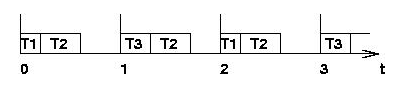
\includegraphics{\imageSrc/clock_ticks.png}
	\caption{Example of periodic tasks: At even clock ticks T1 and T2 are launched at uneven clock ticks T3 and T2.}
	\label{f:perd_ex}
\end{figure}

Using this kind of scheduling doesn't put a 100\% load on the cpu.
The lengths of the task can also varry a little if the sum of durations remains under the clock period.
When calculating the clock period interrupt tasks should be taken into account.

\paragraph{Task synchronisation}
We'll explain a simple form of synchronisation next. 
The idea is that a tasks can suspend the execution of another until a given event.
First the scheduler must be warned that the task has been suspended.
Next some bookkeeping needs to be done in the table of tasks.
Make the appropriate task unrunnable by add a code representing an event that reactives it in the ``lock'' field.
To restart the task another task will have to detect the unlocking event and make the ``lock'' field null again. 
If more locked tasks have the same unlocking event a choice must be made to either unlock the first task (or with highest priority) or all the tasks waiting. 

Other synchronisations can be implemented in a similar way.

\paragraph{Communications}
Two methods can be distinguished communication by shared variables and by messages:
\begin{description}
	\item[by shared variables] It's simple and fast but shared variables must be written mutual exclusively. This makes the tasks strongly synchronised (long waits may occur).
	\item[by messages] The OS acts as a go-between. It can buffer the messages. Mutual exclusion is needed between tasks and OS. Waits can occur when the buffer is full. But messages can also be discarded if necessary an appropriate discarding scheme should then be chosen (often fifo). This buffering cause the tasks to be less synchronized.
\end{description} 


\paragraph{Mutual Exclusion}
On a monoprocessor this can somtimes be achieved with temporarily disabling interrupts.
In any other case this can be implemented by using atomic READ/MODIFY/WRITE assembly language instructions.
On a multiprocessor the memory access between the READ and WRITE will be blocked for all but one processor.
Examples of READ/MODIFY/WRITE instructions are: TSET (test \& set) and ASL (arithmetic shift left). 
For the latter we refer to image \ref{f:asl}. 

\begin{figure}
	\centering
	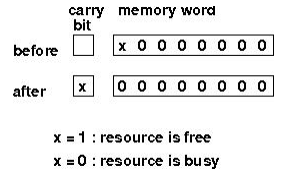
\includegraphics{\imageSrc/ASL.png}
	\caption{Figure showing how Arithmetic Left Shift works.}
	\label{f:asl}
\end{figure}

\subsubsection{Programming}
Which language should be chosen to implement the system layer? 
In general assembly language should be avoided except where it's not possible otherwise (e.g. TSET instruction or tiny programs).
A better choice would be an extensible language (e.g. C or FORTH).
Interactions with the system in such languages goes through functions linked with the program that are not part of the language definition. 
A program can thus be interfaced with any system layer by writing a new set of system interface functions (in the language or assembly).
There are even some dedicated languages for embedded systems. 
These are usually imperative languages including following built-in fuctionallities for:
\begin{itemize}
	\item Hardware Interaction (e.g. interrupt routines).
	\item Multiprogramming management
	\item interprocess communication
	\item process synchronisation
\end{itemize}
They also have some security improvements over extensible languages.
Because they are usually modular and have those built-in functions, verifications of system interactions and syntax is possible by the compiler.
Examples of dedicated languages are: ADA, MODULA 2 and PEARL

\subsubsection{Deployment}
After programming appropriate executable modules should be made.
Most compilers are designed to make programs that should be run on top of an operating system.
Executables for Embedded systems have often specific memory allocation constraints:
\begin{itemize}
	\item interrupt vectors 
	\item programs to be put in ROM
	\item data 
	\item stack
\end{itemize}
The linker should be able to manage these facts and accept directives specifying the desired location and type of memory the sections of the program should be placed in. 
The following are rules the linker/compiler should take into account:
\begin{itemize}
	\item What parts of the program go in each section. 
	\item Where is each section placed in memory.
	\item Is the section ROM or RAM.
\end{itemize}

\subsubsection{Documentation}
Three main documentation documents are required:
\begin{description}
	\item[For the user] Manual and description of behaviour, functionalities of the program.
	\item[For the system engineer] Guidelines to set up and deploy the program succesfully. 
	\item[For the designer] This should be exstensive documentation of all 6 steps for the designer himself or his possible successors. When documenting a posteriori there is a risk to forget important design decisions or strategic choices by focusing to much on the last implementation details. 

\end{document}
